\label{sec:coherence-metrics}
Topic Coherence measures score a single topic by measuring the degree of semantic
similarity between high scoring words in the topic.  These measurements help
distinguish between topics that are semantically interpretable topics and topics
that are artifacts of statistical inference, see Table \ref{tab:best} for
examples ordered by the UCI measure.  For our evaluations, we consider two new
coherence measures designed for LDA, both of which have been shown to match well
with human judgements of topic quality: (1) The UCI measure \cite{newman10uci}
and (2) The UMass measure \cite{mimno11umass}.

Both measures compute the coherence of a topic as the
sum of pairwise distributional similarity scores over the set of topic
words, $V$.  We generalize this as

$$coherence(V) = \sum_{(v_i, v_j) \in V} score(v_i, v_j, \epsilon)$$
\noindent
where $V$ is a set of word describing the topic and $\epsilon$ indicates a
smoothing factor which guarantees that $score$ returns real numbers.
(We will be exploring the effect of the choice of $\epsilon$; the
original authors used $\epsilon=1$.)

\paragraph{The UCI metric} defines a word pair's score to be the pointwise
mutual information (PMI) between two words, i.e.

$$score(v_i,v_j,\epsilon) = \log \frac{p(v_i, v_j) + \epsilon}{p(v_i)p(v_j)}$$
\noindent
The word probabilities are computed by counting word co-occurrence frequencies
in a sliding window over an external corpus, such as Wikipedia.  To some degree,
this metric can be thought of as an external comparison to known semantic
evaluations.

\begin{figure*}[h!t!b!]
  \centering
  \subfloat[UMass]{\label{fig:mean-umass}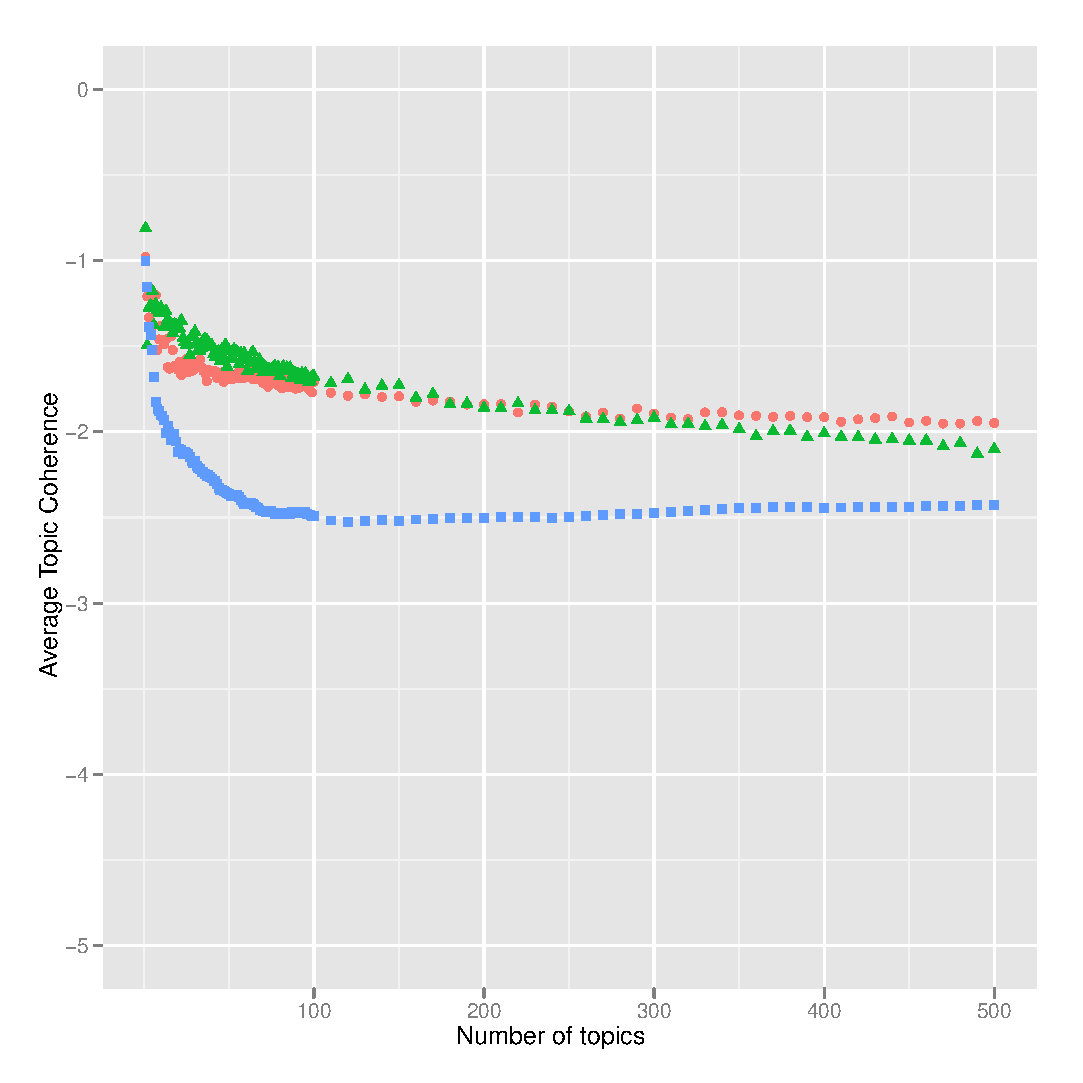
\includegraphics[width=.50\textwidth,height=.35\textwidth]{plots/mean-umass.eps}}
  \subfloat[UCI]{\label{fig:mean-uci}\includegraphics[width=.50\textwidth,height=.35\textwidth]{plots/mean-uci.eps}}
  \caption{Average Topic Coherence for each model}
  \label{fig:mean}
\end{figure*}

\begin{figure*}[h!t!b!]
  \centering
  \subfloat[UMass]{\label{fig:entropy-umass}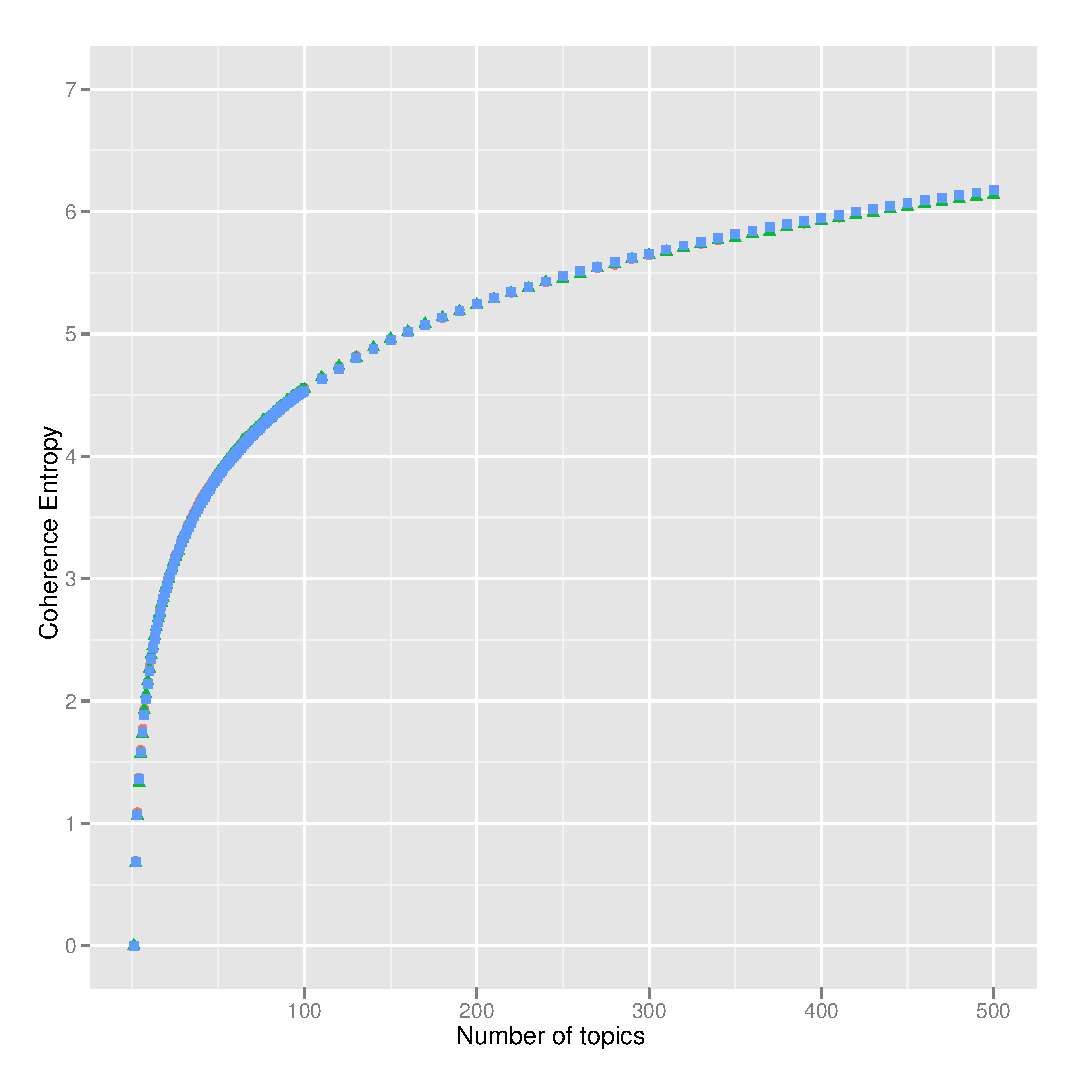
\includegraphics[width=.50\textwidth,height=.35\textwidth]{plots/entropy-umassNoLog.eps}}
  \subfloat[UCI]{\label{fig:entropy-uci}\includegraphics[width=.50\textwidth,height=.35\textwidth]{plots/entropy-uciNoLog.eps}}
  \caption{Entropy of the Topic Coherence for each model}
  \label{fig:entropy}
\end{figure*}

\paragraph{The UMass metric} defines the score to be based on document co-occurrence:

$$score(v_i, v_j,\epsilon) = \log \frac{D(v_i, v_j) + \epsilon}{D(v_j)}$$
\noindent
where $D(x,y)$ counts the number of documents containing words $x$ and $y$ and
$D(x)$ counts the number of documents containing $x$. Significantly, the UMass
metric computes these counts over the \textit{original corpus} used to train the
topic models, rather than an external corpus.  This metric is more intrinsic in
nature.  It attempts to confirm that the models learned data known to be in the
corpus.
